\documentclass[a4paper,12pt]{article} 
\usepackage[utf8x]{inputenc} 
\usepackage[french]{babel} 
\usepackage[colorlinks=true,urlcolor=blue,linkcolor=blue]{hyperref}
\usepackage[T1]{fontenc}
\usepackage[cm]{fullpage}
\usepackage{url}

\usepackage{graphicx}
\usepackage{float}
\usepackage[toc,page]{appendix}


\renewcommand{\appendixtocname}{Annexes}
\renewcommand{\appendixpagename}{Annexes} 
\addto\captionsfrench{\def\tablename{{Tableau}}}
\begin{document}

\title{Analyse des besoins et tests pour le projet\\
  \textit{Réalisation d'un jeu d'Othello}}

\author{Morgane Badré\\
  Benjamin Letourneau,\\
  Vincent Wilmet,\\
  Nicolas Yvon\\}
\date{}

\maketitle

Ce document présente une version préliminaire de l'architecture de notre projet.

\section{Architecture du projet}
Le projet à développer est conséquent, certains modules à réaliser sont plus compliqués que d’autres donc nous avons pensé segmenter en différentes briques. Le principe de la segmentation (voir figure \ref{glob}) en module est qu’ils sont tous indépendants et peuvent être testés indépendamment. Les blocs IA et logiciel sont les plus importants alors que la gestion de fichiers, l’interface et l'éditeur de plateau sont les moins importants. Le second intérêt de cette architecture est que chaque module peut être remplacé par un autre plus ou moins équivalent sans compromettre l’intégrité et le bon fonctionnement du logiciel. Par exemple, pour le bloc de l’IA, si une personne de la communauté souhaite l’améliorer, il peut tout simplement coder le module IA et l’intégrer au logiciel pour le tester. 

Développant en JAVA, les différents modules sont liés par le biais d’interfaces. Ainsi, chaque module présentera une interface définie et dûment commentée qui représentera le comportement du module.


\begin{figure}[H]
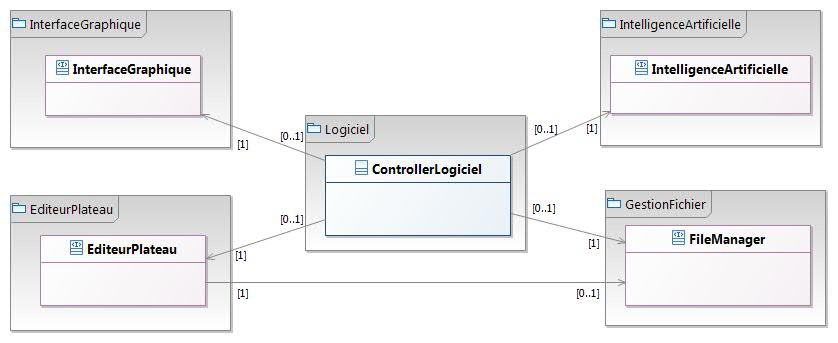
\includegraphics[scale=0.65]{ArchiProjet.jpg}
\caption{Diagramme de classe du projet global}
\label{glob}
\end{figure}

\subsection{Module Logiciel}

Il reprend trois design pattern : State, Factory, MVC.
\begin{itemize}
  \item State sera utilisé pour coder les différents types de pion sur le plateau
  \item Factory sera utilisé pour la génération d’objets
  \item Et l’architecture complète du logiciel sera en MVC pour la maintenabilité et la facilité de lecture/modification du code.
\end{itemize}



\subsection{Module d'Intelligences Artifcielles}

Ce module (voir figure \ref{ia}), le plus compliqué et plus important à réaliser dans notre projet, reprend le design pattern strategy. En effet, on représentera les différents types d’IA en strategie : naïve, force brute, évolutive, ...

\begin{figure}[H]
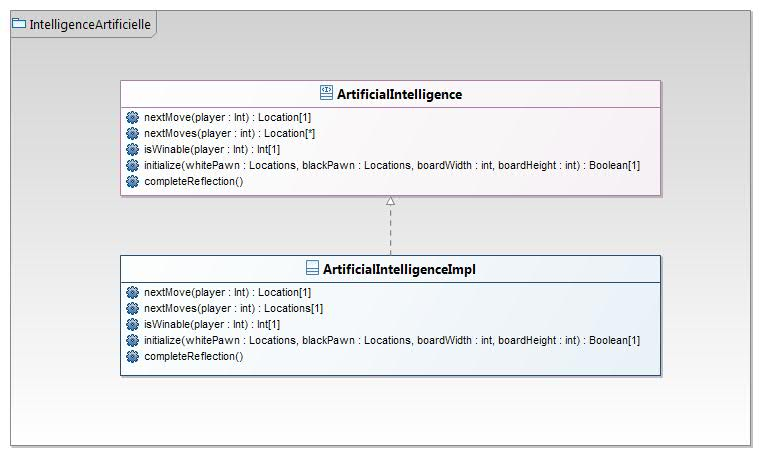
\includegraphics[scale=0.65]{IntelligenceArtificielle.jpg}
\caption{Diagramme UML de classe du module d'intelligence artifcielle}
\label{ia}
\end{figure}

\subsection{Module de Gestion de Fichier}

La gestion de fichiers (voir figure \ref{gest}) ne contient pas de design pattern spécifique.

\begin{figure}[H]
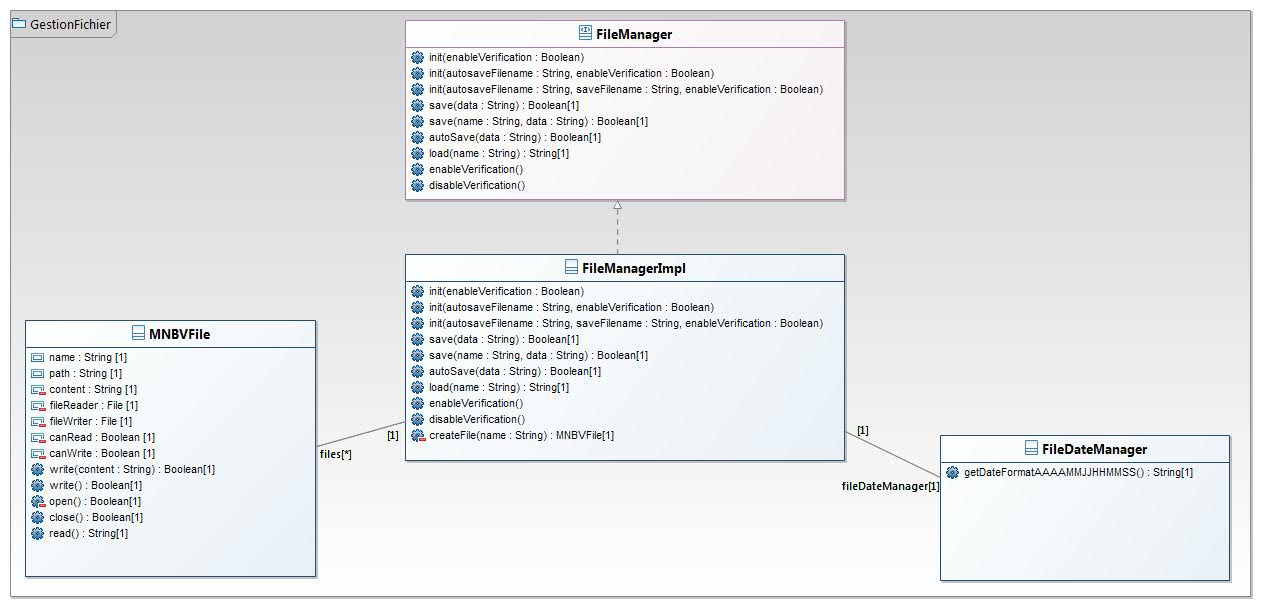
\includegraphics[scale=0.42]{GestionFichiers.jpg}
\caption{Diagramme UML de classe du module de gestion de fichier}
\label{gest}
\end{figure}

\subsection{Module d'Interface Homme-Machine (IHM)}

L’IHM ne contient pas de design pattern spécifique.


\subsection{Module d'Editeur de Plateau}

Ce module (voir figure \ref{edit}) n'utlisera pas de design pattern car si cette fonctionnalité est implémentée, elle ne sera pas forcément graphique mais plus probablement utlisable par la console donc l'architecture sera simple. 


\begin{figure}[H]
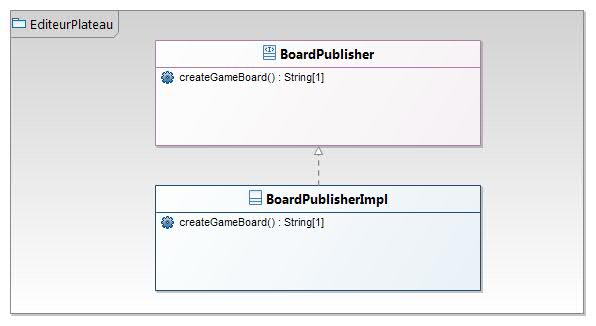
\includegraphics[scale=0.75]{EditeurPlateau.jpg}
\caption{Diagramme de classe du module éditeur de plateau}
\label{edit}
\end{figure}







\end{document}


